\chapter{Background : Effective field theory approach}
In explaining natural phenomena, the separation of scales plays an important role. For instance, to explain the dynamics of gasses, we use a set of macroscopic variables such as pressure, volume, and temperature, which do not provide insight about the molecular (microscopic) structure of the gas molecules. The molecular description of gas is not useful to explain the most day to day phenomena. The microscopic nature of the molecules is needed to understand the chemical structure of these atoms \cite{Petrov:2016azi}. In the above example, the macroscopic view of gasses is the effective theory of the microscopic picture. This effective approach is prevalent in many branches of Physics. As another example, in the quantum mechanical (QM) description of a hydrogen atom does not involve in dynamics of quarks and gluons inside the proton. However, if we zoom in to the hydrogen nucleus, then the dynamics of the quarks and gluons inside the proton becomes essential. More rigorously, the term ``zoom in" can be thought of as an increase in the energy scale that is being probed.\par

\section{Operator product expansion (OPE)}
The effective description of a decay process is given by the effective Hamiltonian. For instance, consider the effective Hamiltionian for $\beta$ decay,
\begin{eqnarray}\label{eff_fermi_int}
\mathcal{H}_{e f f}^{(\beta)}=\frac{G_{F}}{\sqrt{2}} \cos \theta_{c}\left[\bar{u} \gamma_{\mu}\left(1-\gamma_{5}\right) d \otimes \bar{e} \gamma^{\mu}\left(1-\gamma_{5}\right) \nu_{e}\right]
\end{eqnarray}
where equation (\ref{eff_fermi_int}) describe the underlying quark process of the $\beta$ decay and $\theta_c$ is the Cabibbo angle. This effective interaction is shown in figure \ref{fig:fermi_int}.
\begin{figure}[H]
\centering
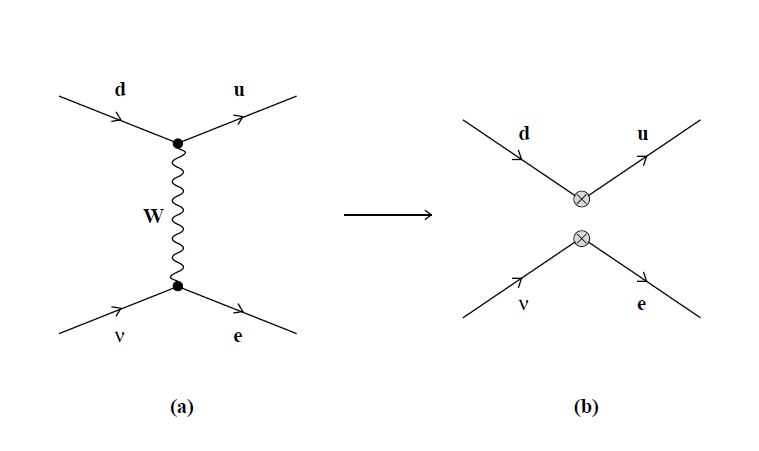
\includegraphics[width=12cm]{fermi_int.JPG}
\caption{\label{fig:fermi_int}
Underlying quark process of $\beta$ decay. (a) represent the SM description and (b) represent the effective representation \cite{Buras:1999rb} .}
\end{figure}
In general, the phenomenology of any weak hadronic decay is given by the following effective Hamiltonian.
\begin{eqnarray}\label{eff_hamiltonian}
\mathcal{H}_{e f f}=\frac{G_{F}}{\sqrt{2}} \sum_{i} V_{\mathrm{CKM}}^{i} C_{i}(\mu) Q_{i}(\mu).
\end{eqnarray}
Here $Q_i$ are relavent local operators that govern the particular decay, $C_{i}(\mu)$ are the Wilson coefficients, which describe the strength of a given operator that enters the Hamiltonian and $V_{\mathrm{CKM}}^{i}$ is the relevent CKM matrix element to the decay. Simply, the equation (\ref{eff_hamiltonian}) can be thought of as a series of vertices multiplied by effective coupling constants $C_i$ \cite{Buras:1999rb}. This effective series is known as an operator product expansion (OPE) \cite{Wilson:1969zs, Wilson:1972ee,Zimmermann:1972tv}. The local operators (vertices) in the OPE involved with the strong and weak interactions, and they can be classified with respect to the Dirac structure, color structure and the type of quarks and leptons relevant for the decay.
\subsection{OPE for B meson decays}\label{section:OPE_b}
The $B$ meson is a bound state of a $b$ quark and a parton (light quark). The decay of $B$ is governed by the processes that involve $W, Z$ and $t$ quark, and they represent the physics at short distance (high energy) scales $\mathcal{O}(M_{W,Z}, m_t)$. At the long distance (energy$\sim \Lambda_{\text{QCD}}$) scale, the hadronization process govern the decay since $\alpha_s(\Lambda_{\text{QCD}})\sim \mathcal{O}(1)$, where at $\Lambda_{\text{QCD}}$ the nonperturbative effects become prominent. The hadronic decay at $\mathcal{O}(m_b)$ is given by effective point like vertices, which are represented by local operators $Q_i$. The Wilson coefficients can be thought of as the coupling constants associated with these $Q_i$.\par 
For instance, the non-leptonic $B$ meson decays involve the following set of local operators.
\begin{eqnarray}
\begin{array}{l}{\text { Current-Current: }} \\ {\qquad Q_{1}=\left(\bar{c}_{\alpha} b_{\beta}\right)_{V-A}\left(\bar{s}_{\beta} c_{\alpha}\right)_{V-A} \quad Q_{2}=(\bar{c} b)_{V-A}(\bar{s} c)_{V-A}}\end{array}
\end{eqnarray}
\begin{eqnarray}
\begin{array}{l}{\text { QCD-Penguins : }} \\ {\qquad Q_{3}=(\bar{s} b)_{V-A} \sum_{q=u, d, s, c, b}(\bar{q} q)_{V-A} \quad Q_{4}=\left(\bar{s}_{\alpha} b_{\beta}\right)_{V-A} \sum_{q=u, d, s, c, b}\left(\bar{q}_{\beta} q_{\alpha}\right)_{V-A}}\\{\qquad Q_{5}=(\bar{s} b)_{V-A} \sum_{q=u, d_{s}, c, b}(\bar{q} q)_{V+A} \quad Q_{6}=\left(\overline{s_{\alpha}} b_{\beta}\right)_{V-A} \sum_{ q=u, d_{s}, c, b}\left(\bar{q}_{\beta} q_{\alpha}\right)_{V+A}}\end{array}
\end{eqnarray}
\begin{eqnarray}
\begin{array}{l}{\text { Electroweak-Penguins : }} \\ {Q_{7}=\frac{3}{2}(\bar{s} b)_{V-A} \sum_{q=u, d, s, c, b} e_{q}(\bar{q} q)_{V+A} \quad Q_{8}=\frac{3}{2}\left(\bar{s}_{\alpha} b_{\beta}\right)_{V-A} \sum_{q=u, d, s, c, b} e_{q}\left(\bar{q}_{\beta} q_{\alpha}\right)_{V+A}} \\ {Q_{9}=\frac{3}{2}(\bar{s} b)_{V-A} \sum_{q=u, d, s, c, b} e_{q}(\bar{q} q)_{V-A} \quad Q_{10}=\frac{3}{2}\left(\bar{s}_{\alpha} b_{\beta}\right)_{V-A} \sum_{q=u, d, s, c, b} e_{q}\left(\bar{q}_{\beta} q_{\alpha}\right)_{V-A}}\end{array},
\end{eqnarray}
where $\alpha$ and $\beta$ are corresponding color indices, $e_q$ is the electric charge of quarks. The operators $Q_2, Q_{3-6}$ and $Q_7, Q_9$ are generated due to the tree level $W^{\pm}$ exchange, gluon penguin and $\gamma, Z^0$ penguin diagrams respectively.
The Wilson coefficients provide the contribution of the short distant ( energy scale higher than $\mu$ ) physics.  Since QCD is asymptotically free, these Wilson coefficients can be  perturbatively calculated. The $C_i$ include the contributions from the $t$ quark, $W$, $Z$, Higgs and SM extensions. In general, Wilson coefficients depend on $m_t$ and the masses of new particles from SM extensions.\par
The scale $\mu$ separates the physics contribution to the decay amplitude to long distance and short distance. Short distance physics governs the interaction at energies that are higher than the value of $\mu$. Whereas, long distance physics governs the interaction at the energies lower than the value of $\mu$. In practice $\mu$ is chosen at the order of $m_b$ (mass of the decaying hadron). Since $\mu = \mathcal{O}(m_b)\gg \Lambda_{\text{QCD}}$, the $C_i$ can be calculated perturbatively in $B$ decays.\par
Long distance physics are contained in local matrix elements $\langle Q_i(\mu)\rangle$. Using the \textit{renormalization group equation} (RGE) we evolve the scale from $\mu=\mathcal{O}(M_W)$ down to $\mathcal{O}(m_b)$. The full amplitude is independent of $\mu$, and it implies the cancellation of the $\mu$ dependence in $C_i$ with the $\mu$ dependence of $\langle Q_i(\mu)\rangle$.
\vspace{-0.4cm}
\subsubsection{Inclusive and exclusive $B$ decays}
\vspace{-0.3cm}
\textit{Exclusive} decays imply the measurement of energy and momenta of all the final state particles. Whereas, in \textit{inclusive} decays the probability of particle decay into a sum of final states ($X$) with a given set of global quantum numbers such as energy and momentum is measured.\par
The amplitude for exclusive decays such as $B$ decay in to final states $F=\pi \nu \bar{\nu}, \pi \pi, D K$ is given by 
\begin{eqnarray}\label{BtoFex}
A(M \rightarrow F)=\left\langle F\left|\mathcal{H}_{e f f}\right| B\right\rangle=\frac{G_{F}}{\sqrt{2}} \sum_{i} V_{C K M}^{i} C_{i}(\mu)\left\langle F\left|Q_{i}(\mu)\right| B\right\rangle
\end{eqnarray} 
where $\left\langle F\left|Q_{i}(\mu)\right| B\right\rangle$ are the hadronic matrix elements of operators $Q_i$ between the initial $B$ meson state and the final state $F$. Evaluation of this matrix element is necessary for the calculation of the exclusive amplitude. The Wilson coefficients $C_i(\mu)$ in equation (\ref{BtoFex}) depends on both the scale $\mu$ and the renormalization scheme that was used for local operators. This is calculated in the renormalization group improved perturbation theory. The hadronic matrix elements $\langle Q_i\rangle$ also depend on both $\mu$ and the renormalization scheme. \par
The evaluation of $\langle Q_i(\mu)\rangle$ requires nonperturbative methods such as lattice calculations, the $1/N_c$ expansion ($N_c$ is the number of colors), QCD sum rules, hadronic sum rules, chiral perturbation theory and so on. Also, for some $B$ meson decays these matrix elements can be analyzed using the \textit{heavy quark effective theory} (HQET).\par
The amplitude for an inclusive $B$ decay is given by
\begin{eqnarray}\label{BtoXinc}
A(B \rightarrow X)=\frac{G_{F}}{\sqrt{2}} \sum_{f \in X} V_{\mathrm{CKM}}^{i} C_{i}(\mu)\left\langle f\left|Q_{i}(\mu)\right| B\right\rangle
\end{eqnarray} 
Unlike the exclusive decays, the scheme dependence in inclusive decay matrix elements can be effectively evaluated. Because of this, the cancellation of this scheme dependence with the scheme dependence in $C_i$ can be systematically studied \cite{Neubert:1993ch}. Therefore, studying the inclusive $B$ meson decays become important from the practitioner's point of view.\par
Inclusive decays have two main advantages over exclusive decays. 
\begin{itemize}
\item The bound state related effects such as Fermi motion \cite{Neubert:1993ch} of heavy quark inside the hadron can be systematically described by heavy quark expansion
\item The bound state effects related to the final state hadrons are removed due to the consideration of final state as a sum of hadronic channels. 
\end{itemize}
The second feature is realized due to the application of \textit{quark hadron duality}\cite{Poggio:1975af, Shifman:2000jv}. This suggests that at high energy scales ($\mu$) the cross section of hadronic decays, which are averaged over the energy range, can be approximately given by the cross sections that are evaluated by quark and gluon pertrurbation theory. 

\section{Heavy quark effective theory (HQET)}\label{sec:HQET}
\subsection{Heavy quark symmetry}\label{sec:heavy_quark_sym}
Due to asymptotic freedom \cite{Gross:1973id} at large momentum transfer (short distance scale), the effective coupling constants $C_i$ become small. Whereas at low energy transfer (long-distance scale), the coupling becomes strong, and the process becomes nonperturbative. This property of QCD makes studying the processes that include decay of heavy quarks easier than the processes that include only the light quarks. These nonperturbative phenomena are dominated at the scale $R_{\text{had}}\sim 1/\Lambda_{\text{QCD}}\sim 1\text{ fm}$ \cite{Neubert:1997gu}. This scale also determines the size of the hadrons. When a mass of a quark ($M_Q$) is much larger than the $\Lambda_{\text{QCD}}$ ($M_Q\gg\Lambda_{\text{QCD}}$), then we call it a heavy quark. In the SM $c,\,b$ and $t$ quarks are considered as heavy.\par
The system of heavy quark and light quarks is a bound state, which is complicated to analyze. The typical momentum exchange between these heavy and light constituents are of $\mathcal{O}(\Lambda_{\text{QCD}})$. This bound state of heavy quark and light quarks can be thought of as heavy quark sitting at the center of the strongly interacting cloud of  \textit{partons} (light quarks). The corresponding Compton wavelength ($\lambda_Q$) for a heavy quark is much less than the size of hadron $\lambda_Q\ll R_{\text{had}}$. This means the heavy quark's quantum numbers are resolved at very small distances compared to $R_{\text{had}}$. In contrast, the soft gluons exchanged between the heavy quark and the light quarks are resolved at much larger distances than the heavy quark. Due to this, the light degrees of freedom become blind to the flavor and spin orientation of the heavy quark. These light quarks will only feel the color field generated by the heavy quark, and it is extended over a larger area compared to the scale of the heavy quark. As shown above, this nature of the interactions between heavy quark and the partons provide a clear separation of scales, which makes this bound state a suitable candidate for an EFT analysis.\par 
Since the heavy quark is irrelevant for the effective analysis, we use the limit $M_Q\rightarrow \infty$ in deriving the theory. Also, in this limit, the differences between various hadronic states that have different heavy flavors tend to have the same configuration. In fact, the configuration of these different hadronic states is determined by the configuration of the light quarks. This property provides the relation between the heavy meson states such as $B, D, B^{*} \text { and } D^{*}$ or between the heavy baryon states such as $\Lambda_b$ and $\Lambda_c$. This means if we change the heavy quark with velocity $v$ in the system with another heavy quark with the same four-velocity and different flavor or spin, the configuration of the light quarks remains the same. Both heavy quarks will remain as static \textit{color sources}. Therefore, we obtain a new symmetry in the effective theory, which includes $N_h$ number of heavy quarks. This symmetry is known as \textit{heavy quark symmetry}, and it is $SU(2N_h)$ internal continuous symmetry \cite{Neubert:1997gu}.  

\subsection{Constructing the HQET Lagrangian}\label{sec:HQET_Lag_constr}
Since the presence of the heavy quark is irrelevant for the configuration of light quarks, at low energies, we can construct a low energy theory in which the heavy degrees of freedom does not appear. This is known as the \textit{``integrating out"}.
This integrating out procedure is similar to the above discussed \textit{Fermi theory} of weak interactions. \par
The \textit{heavy quark effective theory} (HQET) is constructed to simplify the complicated interaction between the heavy quark and the partons by the exchange of soft gluons \cite{Eichten:1980mw, Isgur:1989vq, Balzereit:1996yy, Grinstein:1990mj}. The heavy quark masses $M_Q$ is the high energy scale of the theory. Whereas, we construct the theory to study the interactions at the scale of $\Lambda_{\text{QCD}}$.
 As shown in the section \ref{section:OPE_b}, scale $\mu$ separates long distance and short distance physics contributions. The short distance physics are obtained at the energy scales larger than the heavy quark mass. By considering these two limits for the scale $\mu$, we introduce the scale as in the range $\Lambda_{\text{QCD}}\ll\mu \ll M_Q$ \cite{Neubert:1997gu}. \par
Since we assume the heavy quark is static inside the heavy hadron's rest frame, heavy quark's velocity is equal to the hadron's velocity $v$. Therefore, the momentum of the heavy quark inside the bound state is given by
\begin{eqnarray}
p_{Q}^{\mu}=M_{Q} v^{\mu}+k^{\mu},
\end{eqnarray} 
where $v$ is the four-velocity of the heavy meson, and it is given by $v=(1,0,0,0)$. The $v\cdot v=1$ and $k$ is the residual momentum. The $k$ determines the off-shellness of heavy quarks due to the interactions with light partons. This provides $k\sim\Lambda_{\rm{QCD}}\ll M_Q v$. The changes to the heavy quark velocity $v$ due to these soft interactions are small, and they vanish as $\Lambda_{\mathrm{QCD}} / m_{Q} \rightarrow 0$. \par
As shown in \cite{Neubert:2005mu, Petrov:2016azi}  the near on shell Dirac spinor has two large and two small components, using this, the quantum field for the heavy quark can be defined as follows:
\begin{equation}\label{eqn:HQET_param}
Q(x)= e^{-iM_{Q}\upsilon \cdot x}[h_{\upsilon}(x)+H_{\upsilon}(x)].
\end{equation}
Where $h_{\upsilon}(x)=e^{iM_{Q}\upsilon\cdot x}\dfrac{(1+\slashed{\upsilon})}{2}Q(x)$ represents the large ``upper" component and $H_{\upsilon}(x)=e^{iM_{Q}\upsilon.x}\dfrac{(1-\slashed{\upsilon})}{2}Q(x)$ represents the small ``lower" components. These large and small component fields satisfy $\slashed{v} h_{v}=h_{v} \text { and } \slashed{v} H_{v}=-H_v$. Now the full QCD Lagrangian
\begin{eqnarray}
\mathcal{L}_{Q}=\bar{Q}\left(i \slashed{ D}-m_{Q}\right) Q
\end{eqnarray} 
can be re written as follows:
\begin{eqnarray}\label{eqn:HQET_Lag1}
\mathcal{L}_{Q}=\bar{h}_{v} i v \cdot D h_{v}-\bar{H}_{v}\left(i v \cdot D+2 m_{Q}\right) H_{v}+\bar{h}_{v} i \slashed{D}_{\perp} H_{v}+\bar{H}_{v} i \slashed{D}_{\perp} h_{v},
\end{eqnarray}
where $D_{\perp}^{\mu}=D^{\mu}-v^{\mu} v \cdot D$ is the orthogonal component of the covariant derivative to the heavy quark velocity ($v \cdot D_{\perp}=0$). In the rest frame of the heavy quark $D_{\perp}$ only contains the spatial components of the covariant derivative ($D_{\perp}=(0, \vec{D})$).
From equation (\ref{eqn:HQET_Lag1}), we find that $h_{v}$ describes massless degree of freedom. Whereas, the $H_{v}$ describes a heavy degree of freedom with mass $2M_Q$. The third and fourth terms in the equation (\ref{eqn:HQET_Lag1}) describe pair creation and anhilation of heavy quark and heavy anti-quark. These heavy degrees of freedom can be eliminated using the equation of motion. The HQET equation of motion provides
\begin{eqnarray}\label{eqn:HQET_EOM}
\left(i v \cdot D+2 M_{Q}\right) H_{v}=i \slashed{ D}_{\perp} h_{v}
\end{eqnarray}
by solving the equation (\ref{eqn:HQET_EOM}) for $H_{v}$ 
\begin{eqnarray}\label{eqn:HQET_EOM1}
H_{v}=\frac{1}{2 M_{Q}+i v \cdot D} i \slashed{ D}_{\perp} h_{v}
\end{eqnarray} 
This eliminate the small component of the heavy quark field in the equation (\ref{eqn:HQET_Lag1}).
\begin{eqnarray}\label{eqn:HQET_Lag_1}
\mathcal{L}_{\mathrm{eff}}=\bar{h}_{v} i v \cdot D h_{v}+\bar{h}_{v} i \slashed{ D}_{\perp} \frac{1}{2 M_{Q}+i v \cdot D} i \slashed{ D}_{\perp} h_{v}
\end{eqnarray} 
In momentum space the derivatives that are acting on $h_v$ produce powers of residual momentum $k$. Because of $k\ll M_{Q}v$, we expand the equation (\ref{eqn:HQET_EOM1}) in a \textit{Taylor series}. Applying this expansion in equation (\ref{eqn:HQET_Lag_1}):
\begin{eqnarray}
\mathcal{L}_{\mathrm{eff}}=\bar{h}_{v}i v . D h_{v}+\bar{h}_{v}\frac{i \slashed{ D}_{\perp}}{2 M_{Q}}\left(1+\sum_{n=0}^{\infty}\left(-\frac{i v \cdot D}{2 M_{Q}}\right)^{n}\right) i \slashed{ D}_{\perp} h_{v}
\end{eqnarray}
For $n=0$ the above expression can be further simplified using the following identity
\begin{eqnarray}
\slashed{D}_{\perp} \slashed{ D}_{\perp}=g_{\mu \nu} D_{\perp}^{\mu} D_{\perp}^{\nu}-i \sigma_{\mu \nu} D_{\perp}^{\mu} D_{\perp}^{\nu}
\end{eqnarray}
where $\sigma_{\mu \nu}=\frac{i}{2}\left[\gamma_{\mu}, \gamma_{\nu}\right]$.
Following from this the resulting Lagrangian is obtained as an expansion in $1/M_{Q}^{n}$.
\begin{eqnarray}\label{Hlag}
{\cal L}_{\rm eff}=\bar{h}_{\upsilon}\left(i\upsilon \cdot D-\dfrac{D^{2}}{2M_{Q}}-\dfrac{g}{4M_{Q}}\sigma_{\mu\nu}G^{\mu\nu}\right)h_{\upsilon}+O\left(\dfrac{1}{M_{Q}^{2}}\right),
\end{eqnarray}
where, $G^{\mu\nu}$ is Chromo-electromagnetic field strength tensor.\par
 In the limit $M_Q\rightarrow \infty$ only the first term in equation (\ref{Hlag}) remains
\begin{eqnarray}\label{eqn:HQET_Lag_Infty}
\mathcal{L}_{\infty}=\bar{h}_{v} i v \cdot D h_{v}.
\end{eqnarray} 
\subsubsection{Operators at order $\mathcal{O}(1/M_Q)$ in the HQET Lagrangian}\label{sec:order_1/M_Q }
\vspace{-0.3cm}
Consider the second and the third terms in equation (\ref{Hlag}). The operator, 
\begin{eqnarray}
\mathcal{O}_{\mathrm{kin}}=\frac{1}{2 M_{Q}} \bar{h}_{v}\left(i D_{\perp}\right)^{2} h_{v} \rightarrow-\frac{1}{2 M_{Q}} \bar{h}_{v}(i \vec{D})^{2} h_{v},
\end{eqnarray}
is the kinematic energy of the heavy quark's residual motion. The operator, $\mathcal{O}_{\mathrm{mag}}$ defined in equation (\ref{eqn:mag_op}) is the color-magnetic coupling between heavy quark spin and gluon field.
\begin{eqnarray}\label{eqn:mag_op}
\mathcal{O}_{\mathrm{mag}}=\frac{g_{s}}{4 M_{Q}} \bar{h}_{v} \sigma_{\mu \nu} G^{\mu \nu} h_{v} \rightarrow-\frac{g_{s}}{M_{Q}} \bar{h}_{v} \vec{S} \cdot \vec{B}_{c} h_{v},
\end{eqnarray}
where $\vec{S}$ are the Pauli spin matrix elements, and $B_{c}^{i}=-\frac{1}{2} \epsilon^{i j k} G^{j k}$, which are the components of color magnetic field. \cite{Pauli:1941zz, Dittrich:1985yb, Lee:2006nc}.\par

\section{Non-relativistic QCD}\label{NRQCD}
HQET describes systems that include a single heavy quark and light partons. In HQET the heavy quark's kinetic energy is considered as a power correction. When considering multiple heavy quarks the strong interaction between them at short distances is determined by a single gluon exchange \cite{Manohar:2000dt}. This gluon exchange is defined by a Coulomb potential, and for $\bar{Q}Q$ in a color single state this potential is an attractive potential. This attractive potential is then compensated by heavy quark kinetic energy. This makes the kinetic energy of the heavy quark field play an important role in stabilizing the heavy mesons. The heavy quark kinetic energy cannot be treated as a power correction. Thus, we use a different power counting scheme in NRQCD compared to HQET. This difference is further illustrated in the following example.\par
Consider the figure \ref{fig:Box_diag_two_glu_ex}, which represents a box diagram with two heavy quarks exchange gauge particles (gluons or photons).
\begin{figure}[H]
\centering
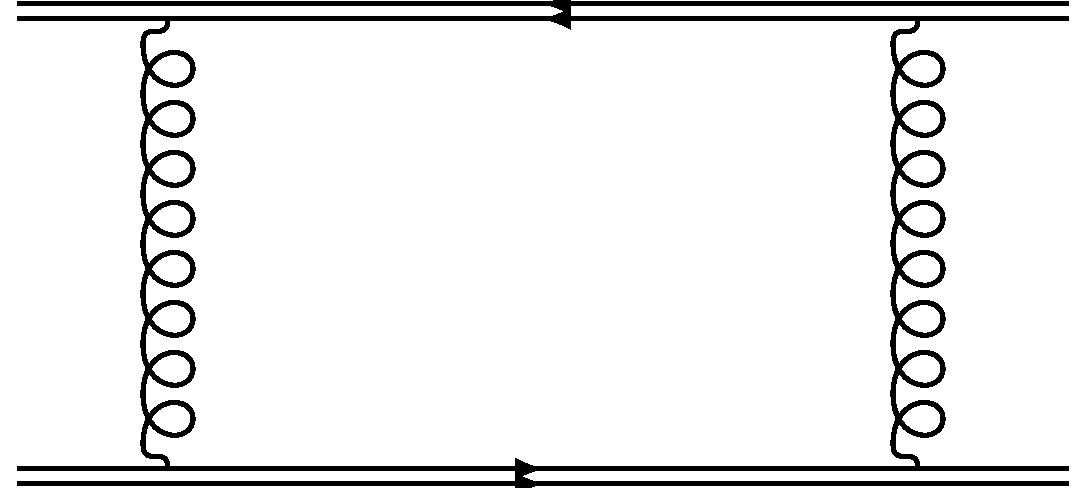
\includegraphics[width=8cm]{box diagram with two heavy quarks1.pdf}
\caption{\label{fig:Box_diag_two_glu_ex}
Box diagram for two heavy quark exchanging gauge particles}
\end{figure}
The integral $I$ that corresponds to the figure \ref{fig:Box_diag_two_glu_ex} is given by \cite{Petrov:2016azi}

\begin{eqnarray}\label{eqn:box_diag_int}
I \sim \int \frac{d^{d} q}{(2 \pi)^{d}} \frac{1}{q^{0}+i \epsilon} \frac{1}{-q^{0}+i \epsilon} \frac{1}{(q+k)^{2}+i \epsilon} \frac{1}{(q-k)^{2}+i \epsilon}
\end{eqnarray}

In the equation (\ref{eqn:box_diag_int}), we find two poles at $q^0=\pm i \epsilon$. These poles are coming from the heavy quark propagators, and they cause a ``pinch singularity". As a result, we cannot deform the contour of the integration without crossing one of these poles \cite{Petrov:2016azi}. To overcome this singularity we need to introduce a new power counting scheme. In this new power counting scheme the importance of the heavy quark kinetic energy is pronounced.\par
In NRQCD the quarkonium is described by an effective Lagrangian, which is expanded as a power series in $v/c$, where $c$ is the vacuum speed of light. The NRQCD Lagrangian can be obtained by using the $c\rightarrow \infty$ limit in the full QCD Lagrangian. 
\subsection{NRQCD Lagrangian}
As shown above, the difference between the HQET and NRQCD is manifested in the first two terms of the effective Lagrangian.
\begin{eqnarray}
\mathcal{L}=Q^{\dagger}(iD^{0})Q+Q^{\dagger}\frac{\bm{D}^2}{2m}Q.
\end{eqnarray} 
In HQET the first term is of $\mathcal{O}(\Lambda_{\rm{QCD}})$ and second term is considered as a correction term of $\mathcal{O}(\Lambda^{2}_{\rm{QCD}}/m)$. Whereas, in NRQCD both terms are of $\mathcal{O}(mv^2)$. Because of this, the heavy quark propagator in both effective theories have different forms. For instance, the heavy quark propagator in HQET is given by $i /\left(k^{0}+i \epsilon\right)$. The NRQCD heavy quark propagator is given by
\begin{eqnarray}\label{eqn:NRQCD_propagator}
\frac{i}{\left(k^{0}-\mathbf{k}^{2} / 2 m+i \epsilon\right)}
\end{eqnarray}
This full NRQCD propagator causes problems in matching calculations. As shown above, the HQET propagator is $m_Q$ independent. Because of this we count the powers of $1/m_Q$ directly from the vertex factors.  For instance, if $s<r$ the effective vertex of $\mathcal{O}(1/m_Q^r)$ does not provide any contribution to terms of $\mathcal{O}(1/m_Q^s)$. Then the matching in HQET is done by expanding Greens function to the desired order in $1/m_Q$. But the NRQCD propagator contains additional power suppressed factors. These factors can wreck the simple power counting of Greens function \cite{Petrov:2016azi}. The solution for this problem is provided in  \cite{Manohar:1997qy}.\par
In \cite{Manohar:1997qy} the full NRQCD propagator is expanded, and the extra terms were treated as a perturbation. The expansion of full NRQCD propagator is given by
\begin{eqnarray}
\frac{1}{k^{0}-\mathbf{k}^{2} / 2 m+i \epsilon}=\frac{1}{k^{0}}+\frac{\mathbf{k}^{2}}{2 m\left(k^{0}\right)^{2}}+\cdots
\end{eqnarray}
The series expansion of propagator prevents the appearance of positive powers of the mass terms. Whereas, the full NRQCD propagator provides these positive powers. Thus, by expanding the NRQCD propagator the NRQCD and HQET matching conditions can be computed using the same procedure.\par
The NRQCD Lagrangian upto dimension seven ($\mathcal{O}(1/m^3)$) is provided in equation (\ref{eqn:NRQCD_Lag_dim_7}). 
This Lagrangian is computed to one loop, and it only considers the terms that are bilinear in fermions \cite{Manohar:1997qy}. In equation (\ref{eqn:Dim_8_Lagrangian}) we provide the dimension eight Lagrangian. This is first obtained in our work \cite{Gunawardana:2017zix}.
 
\section{Applications}
\subsection{Heavy quark spectroscopy}
As shown in the section \ref{sec:heavy_quark_sym}, the dynamics of hadronic bound state with one heavy quark does not depend on its heavy quark's flavor or spin. Because of this, states with different heavy quark flavors can be related to each other. The hadronic states, therefore, are classified by  the quantum numbers of the light degrees of freedom \cite{Falk:1991nq}. From the spin symmetry we find that the total spin of these partons are doubly degenerated with total spin $J=j \pm \frac{1}{2}$ \cite{Isgur:1991wq}.\par
The mass of a hadron $H_Q$ is related to it's heavy quark as follows:
\begin{eqnarray}\label{eqn:quark_hadron_mass_relation}
M_{H_{Q}}=M_{Q}+\bar{\Lambda}+\frac{\Delta M^{2}}{2 M_{Q}}+O\left(1 / M_{Q}^{2}\right), 
\end{eqnarray}
where $\bar{\Lambda}= M_{H_Q}-M_Q$ and $\Delta M^2$ is originated from the order $1/M_Q$ terms in effective Lagrangian. In particular, the mass splitting ($\Delta M^2$) for heavy hadrons are defined as
\begin{eqnarray}\label{eqn:mass_split}
\Delta M^{2}=-\lambda_{1}+2\left[J(J+1)-\frac{3}{2}\right] \lambda_{2},
\end{eqnarray} 
where $\lambda_1$ and $\lambda_2$ are nonperturbative parameters, which parametrize the kinetic energy and the chromo-magnetic interaction of heavy quark in heavy hadron. For instance, consider the $B$ and $B^*$ mesons. These hadronic states are the members of spin doublet $j=\frac{1}{2}$, and they are ground-sate pseudo scalar ($J=0$) and vector ($J=1$) states respectively. Using the equations (\ref{eqn:quark_hadron_mass_relation}) and (\ref{eqn:mass_split}) we obtain
\begin{eqnarray}
M_B&=& M_b+\bar{\Lambda}-\frac{\lambda_1}{2M_b}-\frac{3\lambda_2}{2M_b}\nonumber\\
M_B^*&=& M_b+\bar{\Lambda}-\frac{\lambda_1}{2M_b}+\frac{\lambda_2}{2M_b}
\end{eqnarray}
 Therefore, the mass splitting between these states is given by
\begin{eqnarray}\label{eqn:mass_split_expression}
\begin{aligned} M_{B^{*}}^{2}-M_{B}^{2} &=4 \lambda_{2}+O\left(1 / M_{b}\right) \end{aligned}
\end{eqnarray} 
PDG average for the $B$ and $B^*$ mass spliting is
\begin{eqnarray}
M_{B^{*}}^{2}-M_{B}^{2} = 0.478\pm 0.003 \text{ GeV}^{2}
\end{eqnarray}
From this we obtain 
\begin{eqnarray}  
\lambda_{2} = 0.119\pm 0.001 \text{ GeV}^{2}
\end{eqnarray}
These results are obtained by assuming the $m_b\rightarrow \infty$ limit.\par
The nonperturbative parameter $\lambda_1$ contains the information about ``smearing" in heavy quark momentum \cite{Ball:1993xv}. This parameter is defined as
\begin{eqnarray}
2\lambda_1=-\langle H_Q|\bar{h}_v D^2_{\perp}h_v|H_Q\rangle.
\end{eqnarray}
The $\lambda_1$ can be calculated using the QCD sum rule approch \cite{Ball:1993xv}.Theoretical estimate for the $\lambda_1$ is given in \cite{Gambino:2016jkc}. 